\documentclass[aspectratio=169]{beamer}
\usepackage[utf8]{inputenc}
\usepackage[T1]{fontenc}
\usepackage[portuguese]{babel}
\usepackage{graphicx}
\usepackage{helvet}


\usepackage{tikz}
\usepackage{tikz-3dplot}
\usepackage{amsmath,amssymb}
\usepackage[    backend=biber,
    			style=abnt]{biblatex}

\addbibresource{refs.bib}


\renewcommand{\familydefault}{\sfdefault}


\usetheme[mode=light]{sthlmnord}


\setbeamertemplate{title page}{
	\vfill
	\begin{centering}
		{\usebeamerfont{title}\usebeamercolor[fg]{title}\Huge \textbf{\inserttitle}}\par
		\vspace{1cm}
		{\usebeamerfont{author}\large \insertauthor}\par
	\end{centering}
	\vfill
	\begin{center}
		
\includegraphics[height=1.6cm]{../figures/logo_unespar.png}
		
\includegraphics[height=1.2cm]{../figures/mat.png}
	\end{center}
	\vspace{0.2cm}
}

\setbeamertemplate{footline}{
	\ifnum\insertframenumber>1
	\hbox{%
		\begin{beamercolorbox}[wd=.2\paperwidth,ht=1cm,dp=0.5cm,right,rightskip=0.8cm]{}
			
\includegraphics[height=1.2cm]{../figures/logo_unespar.png}
		\end{beamercolorbox}%
	}
	\fi
}

%Página de título
\title{O conceito de geodésica e o Teorema de Hopf-Rinow na Geometria Riemanniana}
\author{\Large
	João Paulo Chiari de Gasperi\\
	Welinton Anderson Rocha\\
	Roger Emanuel Moraes Pezzott\\
}
\date{}


\begin{document}

% Capa
\begin{frame}[plain]
    \titlepage
\end{frame}

\begin{frame}{Conteúdo}
    \tableofcontents
\end{frame}


\section{Contexto Histórico}

\begin{frame}{Os postulados de Euclides}
    \begin{enumerate}
        \item Fique postulado traçar uma reta a partir de todo ponto até todo ponto.
              \pause
        \item Também prolongar uma reta limitada, continuamente, sobre uma reta.
              \pause
        \item E, com todo centro e distância, descrever um círculo.
              \pause
        \item E serem iguais entre si todos os ângulos retos.
              \pause
        \item E, caso uma reta, caindo sobre duas retas, faça os ângulos interiores e do mesmo lado menores do que dois retos, sendo prolongadas as duas retas, ilimitadamente, encontrarem-se no lado no qual estão os menores do que dois retos (Euclides, p. 98).
    \end{enumerate}
\end{frame}

\begin{frame}{Os postulados de Euclides}
    \begin{block}{Quinto Postulado}
        Dadas duas retas distintas em um plano, caso, traçando uma terceira reta que intercepta ambas, os dois ângulos internos de um mesmo lado da terceira reta, formados interceptando as outras duas retas, somem para menos que 180 graus, então as duas retas se interceptam desse lado.
    \end{block}
    \begin{center}
        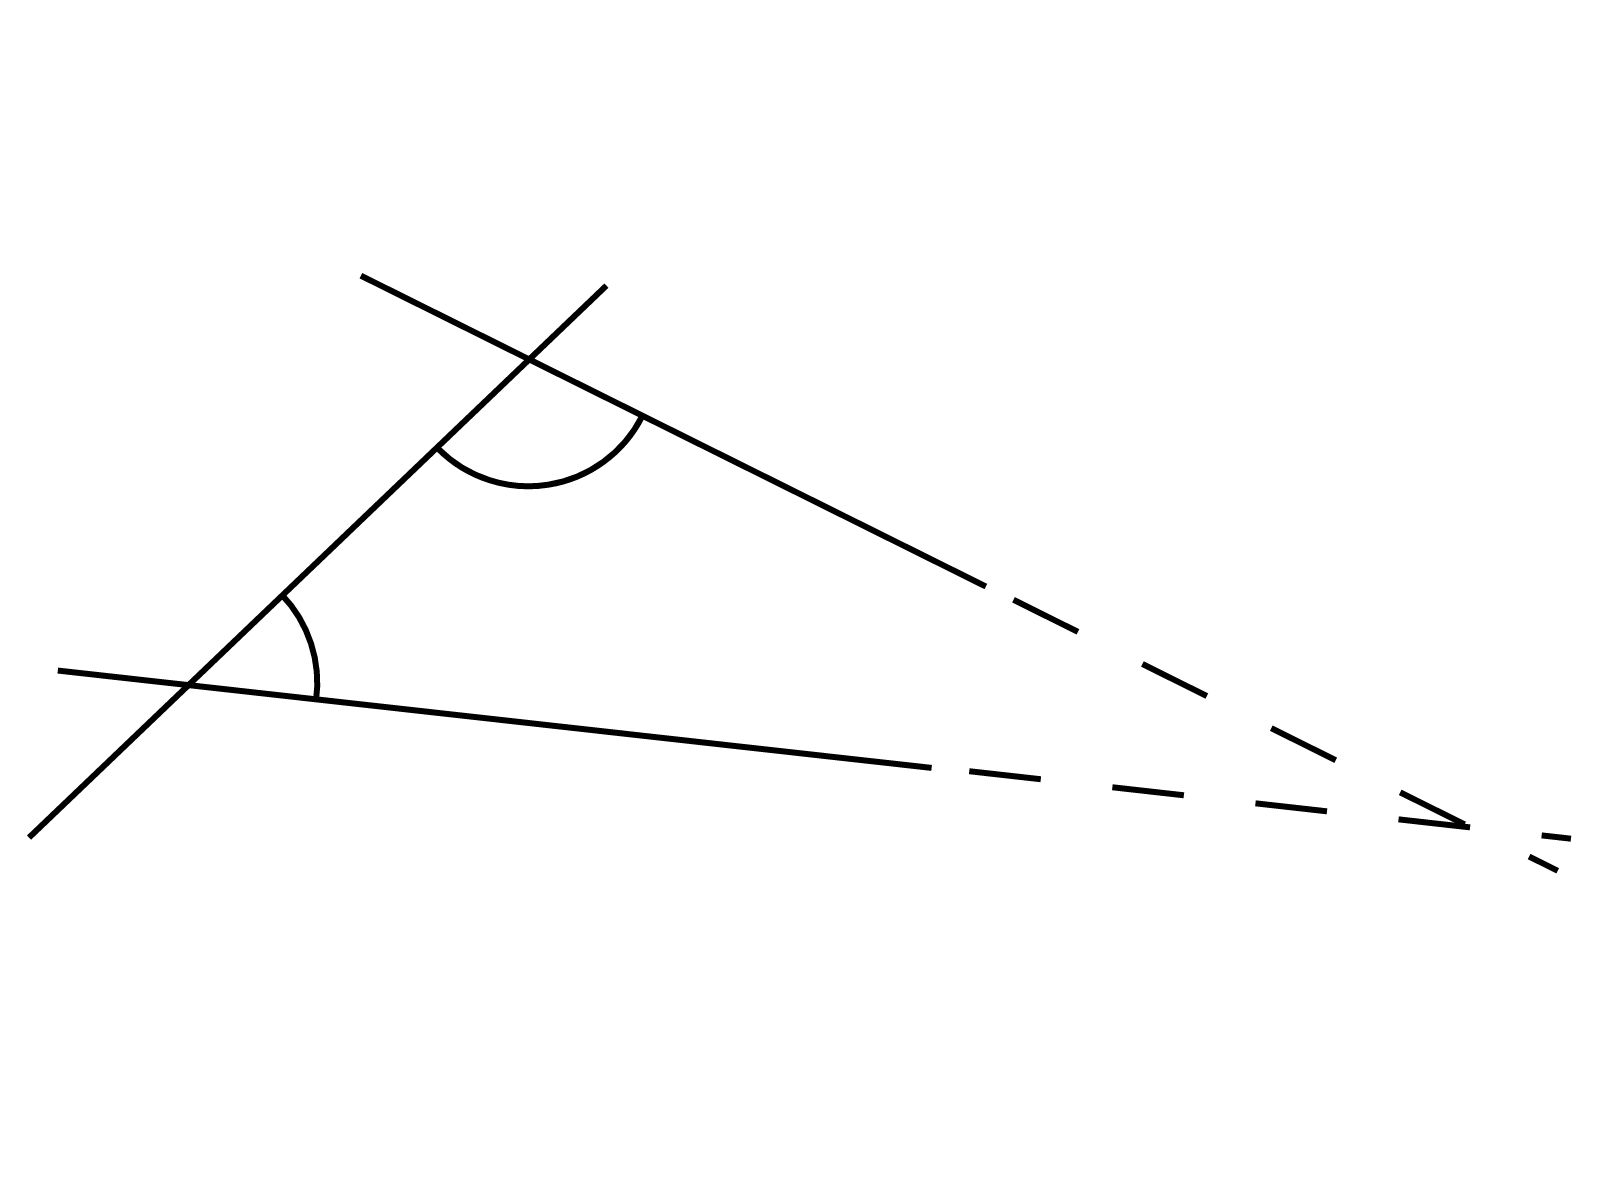
\includegraphics[height=0.5\textheight]{../figures/postulado.png}
    \end{center}
\end{frame}

\begin{frame}{Desenvolvimentos mais recentes}
    \begin{columns}
        \begin{column}{0.3\textwidth}
            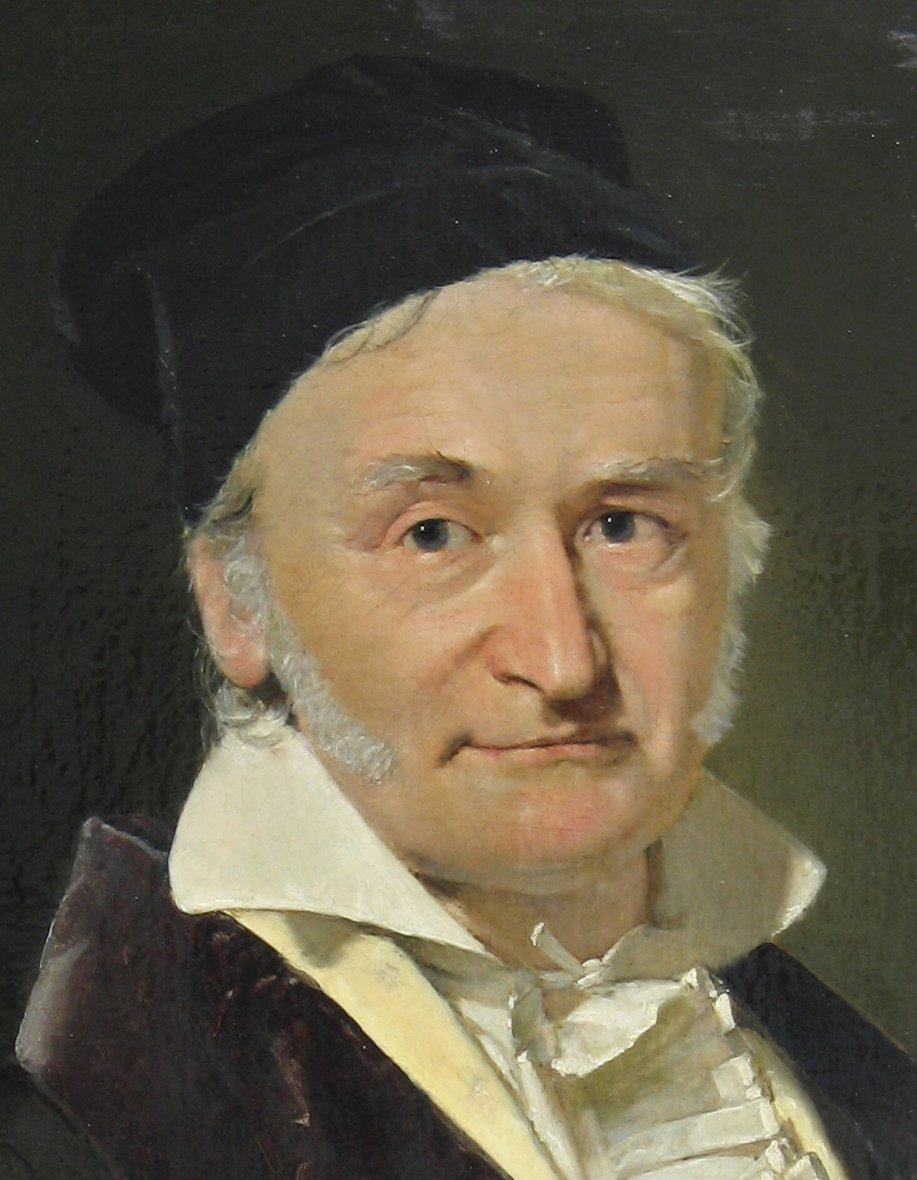
\includegraphics[width=0.8\textwidth]{../figures/gauss.jpg}
            \centering Gauss (1777-1855)
        \end{column}
        \begin{column}{0.3\textwidth}
            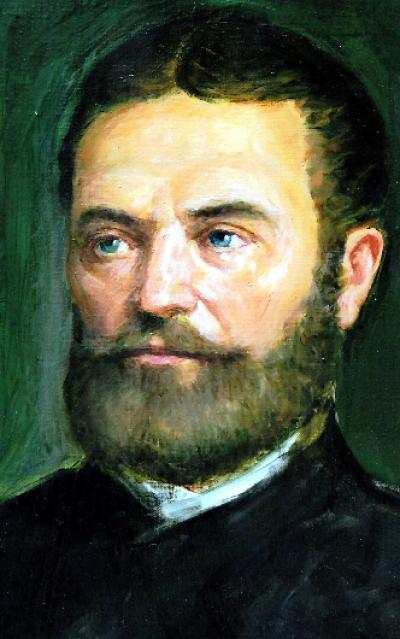
\includegraphics[width=0.8\textwidth]{../figures/bolyai.jpg}
            \centering Bolyai (1802-1860)
        \end{column}
        \begin{column}{0.3\textwidth}
            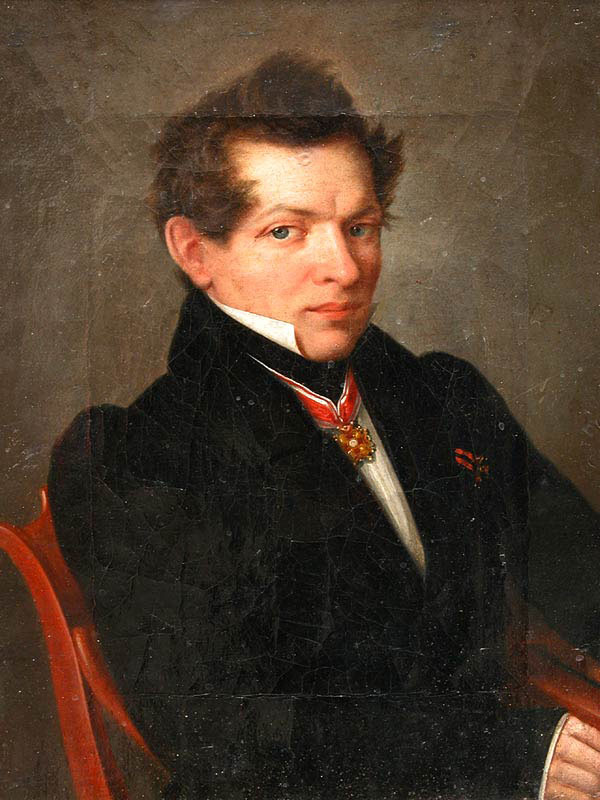
\includegraphics[width=0.8\textwidth]{../figures/lobachevsky.jpg}
            \centering Lobachevsky (1792-1856)
        \end{column}
    \end{columns}
\end{frame}

\begin{frame}{Geometria Diferencial}
    \begin{block}{Objetivo}
        Generalizar conceitos do cálculo para superfícies, as quais são subconjuntos bidimensionais de $\mathbb{R}^3$ e que possuem propriedades diferenciáveis.
    \end{block}
    \pause
    \begin{block}{Resultados e Definições Notáveis}
        \begin{itemize}
            \item Curvatura Gaussiana
            \item Teorema Egregium
            \item Teorema de Gauss-Bonnet
        \end{itemize}
    \end{block}
\end{frame}

\begin{frame}{Geometria Riemanniana}
    \begin{columns}
        \begin{column}{0.3\textwidth}
            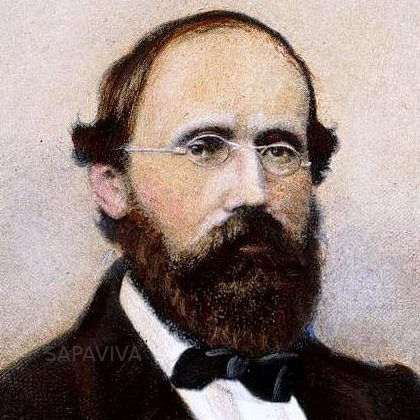
\includegraphics[width=0.8\textwidth]{../figures/riemann.jpg}
            \centering Riemann (1826-1866)
        \end{column}
        \begin{column}{0.65\textwidth}
            \begin{itemize}
                \item Por que se restringir a subconjuntos do $\mathbb{R}^3$?
                      \pause
                \item Podemos generalizar as superfícies para variedades diferenciáveis de dimensão arbitrária.
                      \pause
                \item Tais variedades não precisam ser subconjuntos de $\mathbb{R}^n$.
            \end{itemize}
        \end{column}
    \end{columns}
\end{frame}

\section{Problemática}

\begin{frame}{Geodésicas}
    \begin{block}{Ideia Intuitiva}
        Geodésicas são curvas que generalizam o conceito de reta para variedades diferenciáveis.
    \end{block}
    \pause
    \begin{block}{Exemplo}
        Em uma esfera, as geodésicas são os círculos máximos.
    \end{block}
\end{frame}

\begin{frame}
    \begin{itemize}
        \item Qual é a importância das geodésicas para a compreensão da geometria de variedades riemannianas? \\
        \item Como o Teorema de Hopf-Rinow estabelece a relação entre conceitos locais e propriedades globais desses espaços?
    \end{itemize}
\end{frame}

\section{Objetivos}

\begin{frame}{Objetivos}
    \begin{alertblock}{Geral}
        Estudar o conceito de geodésica e suas principais propriedades no contexto da Geometria Riemanniana, com ênfase no Teorema de Hopf–Rinow.
    \end{alertblock}
    \begin{block}{Específicos}
        \begin{itemize}
            \item Desenvolver a teoria necessária para a formulação e compreensão do Teorema de Hopf–Rinow, incluindo variedades diferenciáveis, métricas riemannianas, conexões afins e geodésicas.
            \item Estruturar os objetos matemáticos estudados e as propriedades desses de forma conexa, lógica e intuitiva.
            \item Construir exemplos que ilustrem os conceitos e resultados estudados, favorecendo a compreensão intuitiva da teoria.
        \end{itemize}
    \end{block}
\end{frame}

\section{Justificativa}

\begin{frame}{Justificativa}
    Relevância matemática do tema, evidenciada pelo seu poder de generalização.
\end{frame}

\begin{frame}{Extensão do conceito de orientabilidade}
    \begin{block}{Exemplos}
        \begin{itemize}
            \item A esfera $S^n$ é orientável.
            \item O toro $T^n$ é orientável.
            \item O plano projetivo $P^2(\mathbb{R})$ não é orientável.
        \end{itemize}
    \end{block}
\end{frame}


\section{Metodologia}

\begin{frame}{Metodologia}
    \begin{alertblock}{Caracterização da pesquisa}
        Essa pesquisa caracteriza-se como bibliográfica, de abordagem qualitativa e natureza dedutiva.
    \end{alertblock}
    \begin{block}{Material a ser estudado}
        \begin{itemize}
            \item Geometria Riemanniana (Do Carmo, 2018)
            \item Introdução à Topologia Diferencial (Lima, 1961).
            \item Outros livros e artigos, conforme surgir a necessidade.
        \end{itemize}
    \end{block}
\end{frame}

\section{Referências}

\begin{frame}[allowframebreaks]{Referências}
    \nocite{*}
    \printbibliography
\end{frame}

\end{document}
